\documentclass[manuscript,screen,review]{jair}

\setcopyright{cc}
\acmDOI{10.1613/jair.1.xxxxx}
\JAIRAE{}
\JAIRTrack{}
\acmVolume{0}
\acmArticle{0}
\acmMonth{0}
\acmYear{2026}

\RequirePackage[
  datamodel=acmdatamodel,
  style=acmauthoryear,
  backend=biber,
  giveninits=true,
  uniquename=init
]{biblatex}
\renewcommand*{\bibopenbracket}{(}
\renewcommand*{\bibclosebracket}{)}
\addbibresource{references.bib}

\usepackage{microtype}
\usepackage{amsmath}
\usepackage{booktabs}
\usepackage{graphicx}
\usepackage{xcolor}
\usepackage[nameinlink,noabbrev]{cleveref}
\usepackage{enumitem}
\usepackage{tikz}
\usepackage{pgfplots}
\usepackage[newfloat]{minted}
\usepackage{csquotes}
\usetikzlibrary{positioning,calc,arrows.meta}

\pgfplotsset{compat=1.18}
\hypersetup{
  colorlinks=true,
  linkcolor=blue!50!black,
  citecolor=blue!50!black,
  urlcolor=blue!50!black,
  pdftitle={Canonical Entity IDs for Grounded Action Generation},
  pdfauthor={J. D. Bohrman}
}

\setminted{
  breaklines=true,
  fontsize=\small,
  bgcolor=black!2,
  frame=lines,
  framesep=2mm
}

\begin{document}

\title[Canonical Entity IDs for Grounded Action Generation]{Canonical Entity IDs for Grounded Action Generation}
\subtitle{A Reference Layer for Small Specialist Models over Structured State}

\author{J. D. Bohrman}
\affiliation{%
  \institution{Independent Researcher}
  \city{New York}
  \state{New York}
  \country{USA}
}
\renewcommand{\shortauthors}{Bohrman}

\begin{abstract}
{\bf Background:}
Small specialist models can produce accurate structured actions when the action schema is narrow and the state is explicit, but they still fail when natural-language instructions refer to entities indirectly. Phrases such as \enquote{the best successor}, \enquote{the highest-confidence track}, or \enquote{the strongest available recon unit} require the model to ground language to one entity among many plausible candidates.

{\bf Objectives:}
We study this problem in a multi-robot coordination setting and test the claim that a stable, consistent, model-facing reference layer can materially improve grounded structured action generation.

{\bf Methods:}
We introduce \emph{Canonical Entity IDs} (CEIDs), a model-facing alias scheme that rewrites domain entities into compact, typed, scope-aware identifiers while preserving a reversible map back to canonical runtime IDs. CEIDs are paired with structured state views, typed action targets, and lightweight ranking hints over candidate entities.

{\bf Results:}
In our harder robotics candidate-pressure slice, a baseline specialist without this reference discipline achieved only 61.6\% exact-match accuracy on a 250-example evaluation. After adding canonical entity IDs, consistent alias rewriting, and ranked grounding hints, the same specialist reached 98.0\% exact-match accuracy, 100\% exact operation accuracy, 100\% valid JSON, and 99.2\% schema validity on the same evaluation slice. The remaining failures are concentrated in a small number of assignment and reassignment cases rather than broad grounding collapse.

{\bf Conclusions:}
These results suggest that reference design is a first-class systems problem for applied AI. Canonical entity IDs provide a simple, inspectable mechanism for improving grounded structured generation without requiring larger base models, broader prompts, or unconstrained agentic reasoning.
\end{abstract}

\maketitle

\paragraph{Code availability.}
Repository, paper source, and released experimental artifacts are available at \url{https://github.com/beaglabs/sst}. The repository code and released dataset artifacts are distributed under the MIT License.

\section{Introduction}
Language models are increasingly asked to issue actions over structured systems rather than write open-ended prose. In such settings, the core problem is often not syntax. It is grounding. A model may know that the requested action is \texttt{reassign\_task} or \texttt{set\_lock\_state}, yet still choose the wrong robot or track because several candidates are semantically plausible.

This failure mode is common in operational domains where the user rarely names the exact identifier they want. Instead, instructions refer to entities by role, quality, or relational status: the best successor, the highest-confidence contact, the strongest available inspection unit. The structured action problem is therefore also a reference problem.

\paragraph{Code availability.}
Repository, paper source, and experimental artifacts are available at \url{https://github.com/beaglabs/sst}.

This paper studies a narrow claim: \emph{small specialist models become materially more reliable when the system gives them a consistent, compact, reversible identity layer over structured state}. We call this layer \emph{Canonical Entity IDs} (CEIDs). CEIDs do not replace structured state or typed actions. They sit between the runtime world and the model, converting entities such as robots, tasks, and tracks into compact model-facing aliases while preserving exact reversibility back to the canonical runtime IDs.

The result is a more legible grounding problem. Instead of forcing the model to reason directly over long heterogeneous identifiers, CEIDs give it a typed, scope-aware vocabulary such as \texttt{robot.recon.w11.a} or \texttt{track.vehicle.w11.2}. Combined with ranking hints over candidate entities, this creates an explicit reference layer for state-to-action generation.

CEIDs also fit naturally into broader specialist-routing systems in which a general controller or interface layer routes user requests to narrow domain models. In such architectures, the routing layer decides \emph{which} specialist to invoke, while CEIDs help the invoked specialist refer to the current entities consistently once it receives structured state.

\paragraph{Contributions.}
\begin{enumerate}[leftmargin=*,itemsep=0.3em]
  \item We define Canonical Entity IDs as a reversible alias layer for structured state-to-action generation.
  \item We show how CEIDs can be integrated into a validator-backed specialist workflow without changing the runtime action schema.
  \item We present a robotics coordination benchmark in which indirect entity references create candidate-pressure grounding failures.
  \item We show that CEIDs plus consistent alias rewriting and ranked grounding hints improve exact-match accuracy from 61.6\% to 98.0\% on a 250-example evaluation slice.
  \item We analyze the main implementation failure encountered during development: inconsistent rewriting between alias-bearing state and helper hints, which temporarily caused a severe schema-validity regression.
\end{enumerate}

\section{Problem Setting}
\subsection{Structured Action Generation}
We study tasks in which a model must map:
\begin{enumerate}[leftmargin=*,itemsep=0.25em]
  \item a natural-language instruction,
  \item a structured state view,
  \item into one typed action object.
\end{enumerate}

The specialist is not asked to emit prose. It is asked to produce one executable edit such as task assignment, task reassignment, robot mode change, or track lock-state update.

\subsection{Why Grounding Fails}
In easy slices, direct references dominate and exact match is straightforward. In harder slices, the instruction deliberately underspecifies the entity and requires model-side resolution from structured state. For example:
\begin{itemize}[leftmargin=*]
  \item \enquote{Assign this task to the strongest available recon unit.}
  \item \enquote{Hand off this task to the best available successor.}
  \item \enquote{Promote the highest-confidence vehicle contact to confirmed.}
\end{itemize}

Without a disciplined reference layer, the model must simultaneously parse the instruction, rank the candidates, and emit the final runtime IDs. In practice this produced the dominant errors in our harder slice.

\section{Canonical Entity IDs}
\subsection{Definition}
A Canonical Entity ID is a model-facing alias with four components:
\[
\texttt{<type>.<class>.<scope>.<slot>}
\]

Examples include:
\begin{itemize}[leftmargin=*]
  \item \texttt{robot.recon.w11.a}
  \item \texttt{robot.inspection.w11.c}
  \item \texttt{task.track.w11.2}
  \item \texttt{track.vehicle.w11.5}
\end{itemize}

Each alias is generated from canonical runtime state and stored with a reversible map. The model sees the aliases; the runtime executes on the original IDs.

\subsection{Design Goals}
The identifier layer is designed to satisfy five properties:
\begin{enumerate}[leftmargin=*,itemsep=0.25em]
  \item \textbf{Typed}: entity kind remains explicit.
  \item \textbf{Compact}: IDs are shorter and more regular than raw runtime identifiers.
  \item \textbf{Scoped}: aliases encode world-local scope rather than pretending to be globally meaningful.
  \item \textbf{Reversible}: every alias has a deterministic reverse mapping to its runtime ID.
  \item \textbf{Model-friendly}: token patterns are regular and semantically grouped.
\end{enumerate}

\subsection{Reference Consistency}
CEIDs are only useful if every model-facing reference path is rewritten consistently. That includes:
\begin{itemize}[leftmargin=*]
  \item candidate ID lists,
  \item candidate entity objects,
  \item target entity objects,
  \item helper summaries and ranking hints,
  \item the instruction itself when it contains direct identifiers.
\end{itemize}

We found this consistency requirement to be operationally important. A temporary bug that left ranking hints in canonical runtime IDs while the rest of the state used CEIDs caused a sharp schema-validity drop despite improving exact-match accuracy. Once the hints were rewritten into the same alias space, performance recovered.

\section{System Overview}
\subsection{Interface Contract}
The full runtime action schema remains unchanged. CEIDs are a model-facing translation layer, not a new execution layer. The specialist still emits typed actions such as:

\begin{listing}[t]
\caption{Representative coordination edit target.}
\label{lst:coordination-edit}
\begin{minted}{json}
{
  "op": "assign_task",
  "taskId": "task.track.w11.2",
  "robotId": "robot.recon.w11.a"
}
\end{minted}
\end{listing}

After generation, the action is resolved back to canonical IDs and checked by a schema/domain validator before execution.

\begin{figure}[t]
\centering
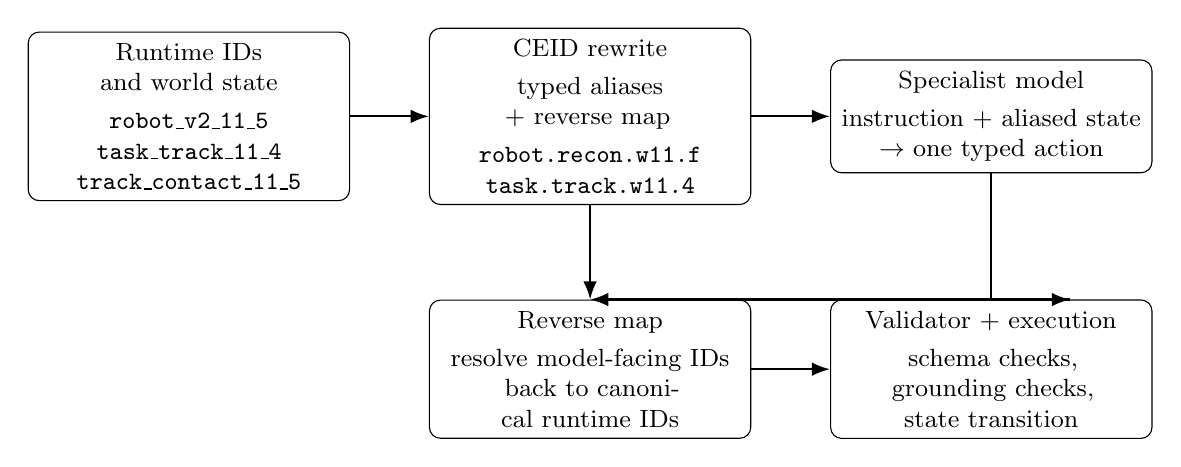
\begin{tikzpicture}[
  node distance=8mm and 10mm,
  box/.style={draw, rounded corners, align=center, text width=38mm, minimum height=12mm, inner sep=4pt, font=\small},
  flow/.style={-Latex, thick}
]
\node[box] (runtime) {Runtime IDs and world state\\[0.3em]\texttt{robot\_v2\_11\_5}\\\texttt{task\_track\_11\_4}\\\texttt{track\_contact\_11\_5}};
\node[box, right=of runtime] (rewrite) {CEID rewrite\\[0.3em]typed aliases + reverse map\\[0.3em]\texttt{robot.recon.w11.f}\\\texttt{task.track.w11.4}};
\node[box, right=of rewrite] (specialist) {Specialist model\\[0.3em]instruction + aliased state\\$\rightarrow$ one typed action};

\node[box, below=12mm of rewrite] (reverse) {Reverse map\\[0.3em]resolve model-facing IDs\\back to canonical runtime IDs};
\node[box, right=of reverse] (validator) {Validator + execution\\[0.3em]schema checks, grounding checks,\\state transition};

\draw[flow] (runtime) -- (rewrite);
\draw[flow] (rewrite) -- (specialist);
\draw[flow] (rewrite) -- (reverse);
\draw[flow] (specialist.south) |- ([xshift=10mm]specialist.south |- reverse.north);
\draw[flow] ([xshift=10mm]specialist.south |- reverse.north) -- (reverse.north);
\draw[flow] (reverse) -- (validator);
\end{tikzpicture}
\Description{A left-to-right pipeline showing runtime IDs and world state flowing into a CEID rewrite step, then into a specialist model. The rewritten IDs also flow into a reverse-mapping step, which combines the model output with the alias map and passes the resolved action to validation and execution.}
\caption{Canonical Entity ID pipeline. Runtime entities are rewritten into model-facing aliases before decoding, then resolved back to canonical IDs before validation and execution. The key requirement is consistency: state views, helper hints, and generated actions must all refer to entities in the same alias space.}
\label{fig:ceid-flow}
\end{figure}


\subsection{Model-Facing State}
\Cref{lst:robotics-state-schema} shows a representative robotics state view. The important addition is the \texttt{selectionHints} block, which contains a small ranked list of likely candidates in the same alias space as the rest of the prompt.

\begin{listing}[t]
\caption{Representative robotics state view with canonical entity IDs and ranking hints.}
\label{lst:robotics-state-schema}
\begin{minted}{json}
{
  "editKind": "set_lock_state",
  "worldMeta": {
    "id": "world_robotics_11",
    "environment": "urban",
    "clockMs": 1716660011000
  },
  "candidateTrackIds": [
    "track.vehicle.w11.1",
    "track.vehicle.w11.2",
    "track.vehicle.w11.3"
  ],
  "candidateTracks": [
    {
      "id": "track.vehicle.w11.2",
      "classification": "vehicle",
      "confidence": 0.91,
      "lockState": "tracking"
    }
  ],
  "selectionHints": {
    "trackSelection": {
      "recommendedTrackIds": [
        "track.vehicle.w11.2",
        "track.vehicle.w11.1",
        "track.unknown.w11.1"
      ]
    }
  }
}
\end{minted}
\end{listing}

\subsection{Validation}
Validation remains central. Each generated action is checked for:
\begin{enumerate}[leftmargin=*,itemsep=0.25em]
  \item JSON parseability,
  \item schema validity,
  \item existence of referenced entities in the current state,
  \item basic domain invariants.
\end{enumerate}

This makes CEIDs compatible with the same validator-backed workflow used by structured specialist systems more broadly. The contribution here is not constrained decoding alone, but a cleaner reference interface for the model \parencite{scholak2021picard,shin2021constrained,geng2023grammar,xia2025structured}.

\section{Experimental Setup}
\subsection{Domain}
We evaluate CEIDs in a synthetic but source-grounded multi-robot coordination domain derived from ROS~2, MAVLink/PX4, and peer-synchronization-inspired abstractions \parencite{ros2_repo,px4_site,iroh_docs,p2panda_site}. The world model contains robots, tasks, tracks, links, and coordination policies. The action space includes:
\begin{enumerate}[leftmargin=*,itemsep=0.25em]
  \item \texttt{assign\_task},
  \item \texttt{reassign\_task},
  \item \texttt{set\_mode},
  \item \texttt{set\_lock\_state}.
\end{enumerate}

\subsection{Harder Candidate-Pressure Slice}
The paper focuses on the harder \texttt{hard\_v2} slice rather than the earlier frozen baseline because the hard slice exposes the grounding problem directly. Candidate choice depends on battery, link quality, role fit, GPS degradation, and task constraints. Instructions often refer to entities indirectly rather than by exact runtime name.

\subsection{Training Setup}
We fine-tune a Qwen2.5-Coder-1.5B base model with LoRA over structured instruction-state-action triples. The main comparison in this draft is between:
\begin{enumerate}[leftmargin=*,itemsep=0.25em]
  \item a baseline structured specialist without the final CEID stack,
  \item the same specialist with CEIDs, consistent alias rewriting, and ranked grounding hints.
\end{enumerate}

The current experiments emphasize exact structured action generation rather than broad language quality. The reported Modal training configuration uses Qwen2.5-Coder-1.5B with LoRA (`r=8`, `alpha=16`, `dropout=0.05`), learning rate `5\times10^{-5}`, warmup `100`, maximum sequence length `3072`, `3` epochs, per-device batch size `4`, and gradient accumulation `4` on a single Modal A100-80GB GPU. Training uses the split files `train.jsonl`, `val.jsonl`, and `test.jsonl` with `7506`, `834`, and `1660` examples respectively. Model selection is by lowest validation loss with evaluation and checkpoint saving every `200` steps and logging every `50` steps. For reproducibility, training fixes the random seed at `42` across Python `random`, NumPy, and PyTorch, and passes the same value as both the trainer seed and data seed. The reported held-out slice is evaluated remotely on Modal on an A10G GPU with deterministic decoding (`temperature=0.0`, `top_p=1.0`, `do_sample=False`, `max_new_tokens=96`) and a cap of `250` held-out examples. All reported results are from a single seed-42 run unless otherwise stated.

\section{Results}
\subsection{Main Quantitative Result}
\Cref{tab:robotics-hard-v2-results} summarizes the current 250-example evaluation slice as a cumulative ablation over the identity-layer stack. Each row adds one change on top of the previous row.

\begin{table}[t]
\centering
\caption{Robotics hard\_v2 cumulative ablation on 250 held-out examples. Each row adds one change on top of the previous row.}
\label{tab:robotics-hard-v2-results}
\begin{tabular}{lcccc}
\toprule
Variant & Valid JSON & Valid Schema & Exact Op & Exact Match \\
\midrule
Baseline specialist & 1.000 & 0.992 & 1.000 & 0.616 \\
Baseline + CEIDs and ranked hints & 1.000 & 0.856 & 1.000 & 0.660 \\
Prior row + consistent hint rewriting & 1.000 & 0.980 & 1.000 & 0.968 \\
Prior row + parser and action normalization & 1.000 & 0.992 & 1.000 & 0.980 \\
\bottomrule
\end{tabular}
\end{table}

The progression matters more than any single row. The baseline specialist already had perfect operation selection, but failed on entity grounding. Adding CEIDs and ranked hints improved exact match immediately, but exposed a consistency bug because the helper hints were still written in canonical runtime IDs rather than CEIDs. Once those hints were rewritten into the same alias space as the rest of the prompt, exact match jumped from 66.0\% to 96.8\%. A final parser and action normalizer cleaned up the remaining generation drift, yielding 98.0\% exact match with 99.2\% schema validity.

\subsection{Failure Evolution}
The development path is informative:
\begin{enumerate}[leftmargin=*,itemsep=0.25em]
  \item The baseline specialist selected the right operation but often the wrong entity.
  \item Adding ranked hints improved exact match but briefly damaged schema validity because the hints were not rewritten into CEIDs.
  \item Fixing hint rewriting restored consistency and produced a large jump in exact match.
  \item A final parser and action normalizer cleaned up residual generation drift such as appended garbage tokens and slight field-shape errors.
\end{enumerate}

\subsection{What the Remaining Failures Mean}
At 98.0\% exact match on this slice, the remaining errors are small and concentrated. They no longer reflect broad grounding collapse. Instead they are rare assignment/reassignment misses or residual generation artifacts. This is a materially different regime from the starting point.

\section{Discussion}
\subsection{Why CEIDs Help}
The simplest explanation is that CEIDs reduce the entropy of reference resolution:
\begin{enumerate}[leftmargin=*,itemsep=0.25em]
  \item aliases are shorter and more uniform than runtime IDs,
  \item entity type is always explicit,
  \item scope is local and regular,
  \item ranked hints share the same identifier space,
  \item the reverse map allows clean execution without exposing runtime complexity to the model.
\end{enumerate}

This does not mean CEIDs are a universal substitute for better modeling. It means that in structured action settings, naming itself is an interface decision with measurable consequences.

\subsection{Relation to Broader Specialist Systems}
CEIDs fit naturally into a broader specialist architecture in which small models operate over canonical state and typed actions while larger controllers handle routing or user interaction. But the evidence in this draft most directly supports the identity-layer claim, not the entire pluggable-expert story. That narrower contribution is the one this paper makes.

\subsection{Relation to Murmuration}
The broader Murmuration idea remains relevant as a system-level framing for multi-specialist coordination, but CEIDs should be understood as a concrete primitive rather than the whole theory. They help multiple components refer to the same entities consistently. That makes them compatible with Murmuration-style architectures without requiring this paper to prove the entire broader thesis. In that sense, Murmuration is a reasonable higher-level framing for systems composed of many narrow specialists, while CEIDs are one concrete reference mechanism that can make such coordination legible and reliable at the action layer.

\section{Limitations}
\begin{enumerate}[leftmargin=*,itemsep=0.25em]
  \item The current benchmark is synthetic, even though it is structured from source-inspired robotics abstractions.
  \item The strongest quantitative result reported here is on a 250-example held-out slice rather than the full test set.
  \item We currently emphasize one base model family and one primary domain.
  \item The present paper does not yet isolate how much of the gain comes from aliasing alone versus aliasing plus ranked hints.
  \item The residual action normalization step is transparent and small, but it is still a post-generation cleanup layer and should be reported as such.
\end{enumerate}

\section{Next Experiments}
The most useful next experiments are:
\begin{enumerate}[leftmargin=*,itemsep=0.25em]
  \item ablate CEIDs against ranked hints more cleanly,
  \item run the same identity layer in a second non-robotics domain,
  \item test whether CEIDs continue to help under larger candidate sets,
  \item compare against stronger constrained-decoding baselines on the same action targets.
\end{enumerate}

\section{Conclusion}
Canonical Entity IDs provide a simple, reversible reference layer for grounded structured action generation. In a robotics coordination benchmark where the baseline specialist struggled with indirect entity references, CEIDs plus consistent alias rewriting and lightweight ranking hints raised exact-match accuracy from 61.6\% to 98.0\% on a 250-example evaluation slice while preserving fully structured outputs. The main lesson is straightforward: for applied AI systems that act over structured state, reference design is not incidental plumbing. It is part of the model interface, and it can determine whether structured specialists ground reliably or fail under candidate pressure. More broadly, CEIDs appear to be a useful primitive for larger coordinated specialist architectures in which multiple models must act over the same evolving world state.

\printbibliography

\appendix

\section{Reproducibility Checklist for JAIR}

\subsection*{All articles}
\begin{enumerate}[leftmargin=*]
  \item All claims investigated in this work are clearly stated. [yes]
  \item Clear explanations are given how the work reported substantiates the claims. [yes]
  \item Limitations or technical assumptions are stated clearly and explicitly. [yes]
  \item Conceptual outlines and/or pseudo-code descriptions of the AI methods introduced in this work are provided, and important implementation details are discussed. [partially]
  \item Motivation is provided for all design choices, including algorithms, implementation choices, parameters, data sets and experimental protocols beyond metrics. [partially]
\end{enumerate}

\subsection*{Articles containing theoretical contributions}
Does this paper make theoretical contributions? [no]

\subsection*{Articles reporting on computational experiments}
Does this paper include computational experiments? [yes]
\begin{enumerate}[leftmargin=*]
  \item All source code required for conducting experiments is included in an online appendix or will be made publicly available upon publication of the paper. [yes]
  \item The source code comes with a license that allows free usage for reproducibility purposes. [yes]
  \item The source code comes with a license that allows free usage for research purposes in general. [yes]
  \item Raw, unaggregated data from all experiments is included in an online appendix or will be made publicly available upon publication of the paper. [partially]
  \item The unaggregated data comes with a license that allows free usage for reproducibility purposes. [yes]
  \item The unaggregated data comes with a license that allows free usage for research purposes in general. [yes]
  \item If an algorithm depends on randomness, then the method used for generating random numbers and for setting seeds is described in a way sufficient to allow replication of results. [yes]
  \item The execution environment for experiments, and the computing infrastructure used for running them, is described in enough detail to allow replication. [yes]
  \item The evaluation metrics used in experiments are clearly explained and their choice is explicitly motivated. [partially]
  \item The number of algorithm runs used to compute each result is reported. [yes]
  \item Reported results have not been cherry-picked by silently ignoring unsuccessful or unsatisfactory experiments. [partially]
  \item Analysis of results goes beyond single-dimensional summaries of performance to include measures of variation, confidence, or other distributional information. [no]
  \item All hyper-parameter settings for the algorithms or methods used in experiments have been reported, along with the rationale or method for determining them. [partially]
  \item The number and range of hyper-parameter settings explored prior to conducting final experiments have been indicated, along with the effort spent on hyper-parameter optimization. [no]
  \item Appropriately chosen statistical hypothesis tests are used to establish statistical significance in the presence of noise effects. [no]
\end{enumerate}

\subsection*{Articles using data sets}
Does this work rely on one or more data sets (possibly obtained from a benchmark generator or similar software artifact)? [yes]
\begin{enumerate}[leftmargin=*]
  \item All newly introduced data sets are included in an online appendix or will be made publicly available upon publication of the paper. [partially]
  \item The newly introduced data set comes with a license that allows free usage for reproducibility purposes. [yes]
  \item The newly introduced data set comes with a license that allows free usage for research purposes in general. [yes]
  \item All data sets drawn from the literature or other public sources are accompanied by appropriate citations. [yes]
  \item All data sets drawn from the existing literature are publicly available. [yes]
  \item All new data sets and data sets that are not publicly available are described in detail, including relevant statistics, the data collection process and annotation process if relevant. [partially]
  \item All methods used for preprocessing, augmenting, batching or splitting data sets are described in detail. [partially]
\end{enumerate}

\end{document}
